\section{Dynamical Berry's phase and non-linear response} 
\label{chapterberry}
In the previous section, we discussed the advantages of frequency-response derived from the  density matrix EOMs, Eq.~\ref{eomsimple}] over real-time approaches that integrate directly Eq.~\ref{eomsimple}].
    We have also discussed the progress in accounting for electron correlation. In fact, within Green's function theory the inclusion of many-body effects into the expression for the nonlinear optical responses is extremely cumbersome. Furthermore the complexity of these expressions grows with the perturbation order. Therefore it is not surprising that there have been only few isolated attempts of including electron correlation at this level of theory.

    Real-time approaches present the major advantage that electron correlation can be included straightforwardly by adding many-body operators to the Hamiltonian. A further advantage of real-time approaches is that they are non-perturbative in the external fields and therefore one obtains optical susceptibilities at any order without increasing the computational cost and with the only limitation dictated by the machine precision. Finally, whtin a real-time approach, several non-linear phenomena and thus spectroscopic techniques are described by the same EOMs. For instance, by the superposition of several laser fields one can simulate sum- and difference-frequency harmonic generation, or four-waves mixing.\cite{boyd} On the other hand, within a real-time density matrix formalism describing the coupling between light and electrons in extended  periodic system is far from straightforward.

    Here, we present a real-time \ai approach based on a formalism alterative to density matrix and based on an effective Schr\"odinger equation where the coupling between light and electrons in a periodic system is derived from the Berry's dynamical polarisation following the scheme proposed by Souza et al.~\cite{souza_prb}. Before presenting the approach, we briefly discussed the  definition of polarisation in periodic systems. In our approach, we introduce correlation both within the Green's function theory, producing the real-time equivalent of the BSE and within a TD-DFT framework.  
    
\subsection{Why do we need Berry's phase?}
%In this work we use dynamical Berry's phase to calculate the non-linear response in extended systems. 
%\begin{wrapfigure}{r}{0.5\textwidth}
%  \begin{center}
%    
\includegraphics[width=0.4\textwidth]{Figures/wrong_polarization2}
%  \end{center}
%  \caption{Surface contribution to the polarisation in a solid. \label{surfacepol}}
%\end{wrapfigure}
For many years, the correct definition of polarisation in periodic systems remained an unsolved problem in solid state physics. 
Over the years, different wrong definitions of bulk polarisation have been proposed in the literature (see a review in Ref.~\cite{restanotes}).
The definition of polarisation is intrinsically related to the one of the dipole operator, that is a problematic object for extended systems.
%In order to understand the problem, let's start the discussion from the polarisation in isolated systems.
%In a system with open boundary conditions, the dipole operator is well defined and therefore one can write down the polarisation as:
%\be
%\PP = \frac{e \langle \vec \rr \rangle}{V} = \frac{e}{V}\int \vec \rr n (\rr) d \rr,
%\label{polisolated}
%%\ee
%where $n(\rr)$ is the electronic density.
%The simplest idea for the definition of the polarization in periodic systems would be to generalise the previous formula. The integral in Eq.~\ref{polisolated} can be redefined in different possible ways in periodic systems. We can average the dipole operator on the whole material or consider its unit cell. In the first case we obtain $ \PP = \langle \vec \rr \rangle_{sample}/V_{sample}$. In an insulator the contributions from the dipoles inside the material cancel each other (as one can see from  Fig.~\ref{immerse}) and only the surfaces contribute to the total polarisation (see Fig.~\ref{surfacepol}):                              
%\be
%\Delta \PP = \frac{(\Delta \sigma L^2) L }{L ^3},
%\label{polsurface}
%\ee
%where $\Delta \sigma$ is related to the charges accumulated on the surfaces.\cite{vanderbilt1993electric} 
%This definition [Eq.~\ref{polsurface}] is not suitable for numerical calculations because it requires the simulation of the entire sample and moreover the above defined polarisation is not a bulk property but it depends from the surfaces.\\ 
%The second possibility is to define the polarisation as  $ \PP = \langle \vec \rr \rangle_{cell}/V_{cell}$. But this definition is completely arbitrary. In fact different choices of the unit cell give completely different polarisations for the same material, see Fig.~\ref{cellpol}. A last possibility exists, the use of the dipole matrix elements in terms of Bloch orbitals, but also in this case there is problem since the dipole operator is unbounded in periodic systems.\\
%\begin{wrapfigure}{l}{0.5\textwidth}
%    \vspace{-0.7cm}
%%  \begin{center}
%    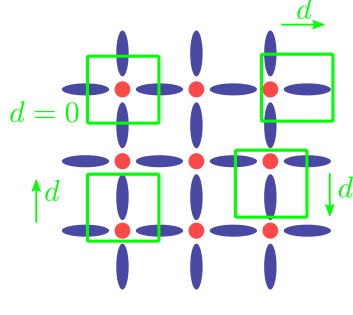
\includegraphics[width=0.4\textwidth]{Figures/wrong_polarization1}
%%%  \end{center}
%  \caption{Polarisation vector versus the choice of the unit cell. \label{cellpol} }
%\end{wrapfigure}
%Finally let mention that also the well know Clausius-Mossotti formula for the polarisability\cite{Mossotti} cannot be used in real solids because wave-functions are not localised objects.\\
In crystalline solids, the definition of bulk polarisation is difficult for two main reasons.
First, in treating crystalline solids one imposes periodic boundary conditions to reflect the periodicity of the lattice and the Bloch functions. With periodic boundary conditions, the position operator is ill-defined. Then, a definition of the dipole operator, and thusoof the polarisanility,  that relies on the position is ill-defined.% in periodic systems, because $\vec \rr$ is not periodic while wave-functions are. WF ARE NOT PERIODIC... BLOCH THEO
Second, differently from finite systems, the polarisation cannot be expressed as an integral on the charge density\cite{Martin1998}.
This can be understood when we write down the general relation between polarisation and density:
\be
\nabla \cdot \PP(\rr) = - n(\rr),
\ee                              
which, for a periodic system, can be written in terms of the Fourier components of $\PP$ and $n$, where $\GG$ denotes a reciprocal lattice vector and $\qq$ belongs to the first Brillouin zone(BZ), as:
\be
(\qq + \GG) \cdot \PP(\qq + \GG) = i n (\qq + \GG).
\label{poldens}
\ee
It follows from Eq.~\ref{poldens} that each Fourier component can be treated separately. Now let us consider the limit $\qq \rightarrow 0$ for $\GG=0$: the macroscopic polarisation $\PP$ is not determined by the zero Fourier component of the density, which must vanish by charge neutrality. In finite systems, this  is fixed by the condition  $\PP(\rr) \rightarrow 0 $ outside the sample (Dirichlet boundary condition). Instead in an infinite crystal, in the limit $\qq = 0$, the polarisation contains additional information not included in the density.\cite{Martin1998} 
A correct definition of polarisation in periodic systems was proposed in 1993 by  King-Smith and Vanderbilt,\cite{KSV1} and later refined by Resta.~\cite{PhysRevLett.80.1800,RevModPhys.66.899}
%
% CHECK: IS CORRECT TO SAY REFINE?
%
In their seminal paper, King-Smith and Vanderbilt showed that the bulk polarisation can be expressed as a closed integral in the Brillouin zone on the wave-function phase, a particular case of the Berry's phase. Their formulation solved all problems with the previous attempts to define the polarisation. In fact the King-Smith and Vanderbilt polarisation is a bulk quantity, its time derivative gives the current and its derivatives respect to the external field reproduce the polarisabilities at all orders.


%*******************************************************************
\subsection{Bulk polarization and response functions}
%% \emph{Ab-initio} approaches based on Green's function theory became a standard tool for quantitative and predictive calculations of linear response optical properties in Condensed Matter. In particular, the state-of-the-art approach combines the $G_0W_0$ approximation for the quasi-particle band structure~\cite{aryasetiawan1998gw} with the Bethe-Salpeter equation in static ladder approximation for the response function.~\cite{strinati} This approach proved to effectively and accurately account for the essential effects beyond independent particle approximation (IPA) in a wide range of electronic systems, including extended systems with strong excitonic effects.~\cite{Onida}

%% In contrast, for nonlinear optics \ai calculations of extended systems rely in large part on the IPA\cite{PhysRevB.48.11705} with correlation effects entering at most as a rigid shift of the conduction energy levels\cite{PhysRevB.80.155205}.  Within time-dependent density-functional theory (TDDFT), it has been recently proposed~\cite{PhysRevB.82.235201} an approach to calculate the second-harmonic generation (SHG) in semiconductors that takes into account as well crystal local-field and excitonic effects. However, this promising approach~\cite{Cazzanelli2012} is limited by the treatment of the electron correlation to systems with weakly bound excitons.~\cite{LRC} 

%% %In fact, it is extremely involved to include many-body effects into the expression for the nonlinear optical susceptibilities within Green's function theory. 
%% %In fact, the inclusion of many-body effects in the equations for the non-linear susceptibilities makes them very difficult to solve.
%% Within Green's function theory the inclusion of many-body effects into the expression for the nonlinear optical susceptibilities is extremely difficult. 
%% Furthermore the complexity of these expressions grows with the perturbation order. Therefore it is not surprising that there have been only few isolated attempts to calculate second-order optical susceptibility using the Bethe-Salpeter equation~\cite{Leitsmann2005,Chang2002} and no attempt to calculate higher-order optical susceptibilities.~\cite{PhysRevB.80.165318} 
%% %The complexity growing with the perturbation order, there have been only few isolated attempts at calculating second-order optical susceptibility using the Bethe-Salpeter equation,~\cite{Leitsmann2005,Chang2002} and in practice third-order optical susceptibility is untreatable.~\cite{PhysRevB.80.165318} 
%% %On the other hand, the origin of this limitation is the attempting to calculate the nonlinear optical susceptibility directly in terms of the electronic structure. 

%% Alternatively to the frequency-domain response-based approach, one can obtain the nonlinear optical susceptibility in time-domain from the dynamical polarisation $\PP$ of the system by using the expansion of $\PP$ in power of the applied field
%% \be
%% \label{eq:peopbf}
%% \PP= \chi^{(1)} \efield + \chi^{(2)} \efield^2 + \chi^{(3)} \efield^3 + \dots 
%% \ee 
%% This strategy is followed in several real-time implementations of TD-DFT\cite{PhysRevB.54.4484}. In these approaches the dynamical polarisation is obtained by numerical integration of the equations of motion (EOMs) for the Kohn-Sham system.\cite{takimoto:154114,castro:3425,meng:054110} %So far applications regard mostly nonlinear optical properties in molecules.  

 
%% The time-domain approach presents three major advantages with respect to frequency-domain response-based approaches. First, many-body effects are included easily by adding the corresponding operator to the effective Hamiltonian. Second, it is not perturbative in the external fields and therefore it treats optical susceptibilities at any order without increasing the computational cost and with the only limitation dictated by the machine precision. Third, several non-linear phenomena and thus spectroscopic techniques are described by the same EOMs. For instance, by the superposition of several laser fields one can simulate sum- and difference-frequency harmonic generation, or four-waves mixing.\cite{boyd}

%% %In a recent work,~\cite{attaccalite} we proposed a real-time implementation of the Bethe-Salpeter equation, based on nonequilibrium Green's function formalism.
%% This approach has shown very promising results for molecular systems, and has been extended to periodic system within the velocity gauge.\cite{tancogne2020octopus,noda2019salmon} However the velocity gauge presents an intrinsic difficulty because non-local operators in the Hamiltonian cannot be easily managed, since they do not commute with the gauge transformation.\cite{tokman} \\
%% Here we present an alternative approach to real-time simulation for extended systems in the length gauge.
%% In this gauge, due to problematic definition of the position operator and polarization, it is not trivial to apply Eq.~\eqref{eq:peopbf} to systems in which periodic boundary conditions (PBC) are imposed. As it was recognised for example in Ref.~\onlinecite{PhysRevB.52.14636}, the same problem appears in the direct evaluation of the nonlinear optical susceptibility in frequency-response based approaches. In particular the dipole matrix elements between the periodic part of the Bloch functions are ill-defined when using the standard definition of the  position operator. In that case, it is possible to obtain correct expressions for the dipole matrix elements from perturbation theory~\cite{PhysRevB.52.14636,PhysRevB.48.11705,PhysRevB.82.235201,korbel2015optical} at a given order in the external field. Instead, in the real-time approach one needs an expression valid at each order of the perturbation.
%% A correct definition of the polarisation operator in systems with PBC has been introduced by means of the geometric Berry phase in the Modern theory of polarisation.\cite{RevModPhys.66.899} 
%% %To our knowledge 
%% Different schemes for calculating the electron-field coupling consistently with PBC have been proposed in Refs.~\cite{springborg, PhysRevB.76.035213, souza_prb, korbel2015optical}. In those works the dipole matrix elements are evaluated numerically from the derivative in the crystal-momentum ($\kk$) space. The latter cannot be carried out trivially because of the freedom in the gauge of the periodic part of the Bloch functions. In fact, the gauge freedom leads to random phases, and random linear combination matricies in degenerate spaces. When considering Bloch functions at two neighbouring $\kk$ points, these random terms needs to be properly accounted for, otherwise spurious contributions to the numerical derivative appear.
%% Then, basically the dfferent schemes~\cite{springborg, PhysRevB.76.035213, souza_prb, korbel2015optical} differ in how these random terms are properly accounted for.

%% Here we will present a real-time \ai approach to nonlinear optical properties for extended systems with PBC in which the nonlinear optical susceptibility are obtained through Eq.~\eqref{eq:peopbf}. To derive the EOMs, and account for the random phases of mixing between different k-points, we follow the scheme of Souza et al.\cite{souza_prb} based on the generalisation of Berry's phase to the dynamical polarisation. Originally applied to a simple tight-binding Hamiltonian, this approach is valid for any single-particle Hamiltonian and it can be applied in an \ai context with inclusion of the relevant many-body effects.\\
%% We will present also a reformulation of the problem in the TD-DFT language, with a functional that depends both on density polariazion. 
%% Finally we will discuss how nonlinear optical susceptibilities are extracted from the dynamical polarisation, and present some results for the second, third harmonic generation and two-photon absorption. \\
%{\color{red} We started with the EOM of the one-body reduced density matrix and on top of it we just discussed TDDFT. We should say few words on why now we are going to change EOM and move to a Lagrangian for QPs. Indeed we are back into a framework for WFs only (i.e. pure states)...}
   
%The Berry phase was introduced in the context of the , a theory that deals with the definition of static bulk polarisation for many-electron correlated systems and noncrystalline systems, by showing that the correct coupling of the electronic wavefunction with the electric field is through a geometric many-body phase operator. 


%% %\textcolor{red}{In the introduction dovremmo discutere anche un po' di non linear optics, citare Sipe, Luppi ed anche Berkaine\cite{PhysRevB.83.245205}, quest'ultimo ha usato la fase di Berry per calcolare la X2 e X3 statica nel TeO2}

%\section{Theoretical background}\label{sc:theory}
%We consider a system of $N$ electrons in a crystalline solid of volume $V=Mv$ (where $M$ is the number of the equivalent cells and $v$ the cell volume) coupled with a time-dependent electric field $\efield$
%\be
%H(t)=H^0 + H^{\efield}(t), \label{eq:startH}
%\ee
%where $H^0$ is the zero-field Hamiltonian, and $H^{\efield}(t)$ describes the coupling with the electric field. % is treated within the dipole approximation ($-e$ is the electronic charge).
%%In this section we do not specify the $H^0$ Hamiltonian but consider a generic one particle Hamiltonian that respects Born-von K\'arm\'an periodic boundary condition.\\
%%To have a computational treatable problem, $H^0$ in Eq.~\eqref{eq:startH} is usually approximated treating the electron-electron interaction through an effective one-particle operator. 
%Here, we consider a generic single-particle Hamiltonian $H^0$. In Sec.~\ref{ss:correff} we specify the form of $H^0$ and show how many-body effects are included by means of effective single-particle operators. Of course, the choice of a single-particle Hamiltonian prevents applications to systems with strong static correlation such as Mott insulators or frustrated magnetic materials.
%%that respects Born-von K\'arm\'an periodic boundary condition.\\
%We assume the ground state of $H^0$ to be non-degenerate and a spin-singlet so that the ground-state wave-function can be expressed as a single Slater determinant. 
%We assume that $H^0$ is such that the many-body ground-state wavefunction can be expressed as a single Slater determinant (see Sec.~\ref{ss:correff}). Of course, this choice prevents applications to systems with strong static correlation.  
%We also assume, as usual in treating cell-periodic systems, Born-von K\'arm\'an PBC and define a regular grid of  $N_\kk=M$  $\kk$-points in the Brillouin zone. With such assumptions, the single-particle solutions of $H^0$ are Bloch-functions.

%Regarding the electron-field coupling we assume classic fields and use the dipole approximation, $H^{\efield}(t)=e\efield(t)\hat r$ ($-e$ is the electronic charge).  However, because of the PBC the position operator is ill-defined. In order to obtain a form for the field coupling operator compatible with  Born-von K\'arm\'an PBC, in this chapter we use the Berry's phase formulation of the position operator and  consequently the polarisation. As proved in Ref.~\cite{souza_prb}, in this formulation the solutions of  $H(t)$ are also in a Bloch function form: $\phi_{\kk,n}(\rr,t) = \mathrm{exp}(i\kk\cdot\rr) v_{\kk,n} (\rr,t)$, with  $v_{\kk,n}$ being the periodic part and $n$ being the band index. Notice that, even in the Berry's phase formulation, for very strong fields and with the number of $\kk$-points that goes to infinity the Hamiltonian Eq.~\ref{eq:startH} is unbounded from below due to the Zener tunnelling.\cite{springborg} Nevertheless the strength of the fields used in non-linear optics is well below this limit.\cite{springborg,souza_prb}\\
%In Sec.~\ref{ss:fldcpl} we detail how, by starting from the Berry's phase formulation of polarisation, we  obtain the EOMs in presence of an external electric field within PBC.  



%*******************************************************************               
\subsubsection{Treatment of the field coupling term and equations of motion}\label{ss:fldcpl}
%In this section we take a different path to obtain the KSV polarisation. 
We sketch the derivation of the EOMs for electrons in a periodic potential coupled with an external electric field in length gauge. We start from the macroscopic bulk polarisation, in terms of the many-body geometric (Berry) phase, as defined in the Modern Theory of Polarisation\cite{RevModPhys.66.899},
%
% CHANGED HERE SINCE WE ALREADY MENTIONED IT - OTHERWISE LOOKED AS THE FIRST TIME - ALSO ADDED BERRY TO CONNECT TO WHAT WE WROTE BEFORE
%
\be 
%\langle X \rangle &=& \frac{L}{2\pi}
%\mbox{Im ln}  \langle \Psi_0 | {\rm e}^{i\frac{2\pi}{L} \hat{X}} | \Psi_0
%\rangle \label{main} \\
%\PP_\alpha =  \lim_{V \rightarrow \infty} \frac{e}{2\pi} \mbox{Im ln }  \langle \Psi_0 | {\rm e}^{i \bb_\alpha \cdot \hat{\mathbf X}} | \Psi_0 \rangle . \label{limit} 
\PP_\alpha =  \frac{e N_{\kk_\alpha} \lv_\alpha}{2\pi V} \mbox{Im ln }  \langle \Psi_0 | {\rm e}^{i \qq_\alpha \cdot \hat{\mathbf X}} | \Psi_0 \rangle . \label{limit} 
\ee
In Eq.~\eqref{limit} $\PP_\alpha$ is the macroscopic polarisation along the primitive lattice vector $\lv_\alpha$, $\hat{\mathbf X} = \sum_{i=1}^{N} \hat{\mathbf x}_i$, $\qq_\alpha = \frac{\bb_\alpha}{N_{\kk_\alpha}}$ with $\bb_\alpha$ the primitive reciprocal lattice vector such that $\bb_\alpha\cdot\lv_\alpha=2\pi$, and $N_{\kk_\alpha}$ the number of $\kk$-points along $\alpha$, corresponding to the number of equivalent cells in that direction, $\qq_\alpha$ is the smallest distance between two k-points along the $\alpha$ direction.
Note that in this formulation the polarisation operator is a genuine many-body operator that cannot be split as a sum of single-particle operators. \\
The polarization defined by the Eq.~\ref{limit} is valid for any many-body wave-function on lattice or continuum\cite{PhysRevLett.80.1800,resta1999electron}. This expression can be simplified in case the full many-body wave-function  $\Psi_0$ can be written as a single Slater determinant.
%% By using the assumption that  to simplify Eq.~\eqref{limit} we assume . 
%% A further simplication comes by specializing Eq.~\ref{limit} for crystalline systems, that is by assuming that our system is composed of $n_{\text{cell}}$ equivalent cells, 
%, where $L=N_{\kk} a$ and $a$ is the lattice vector. 
In this case, the expectation value of the many-body geometric phase in Eq.~\eqref{limit} can be written in terms of overlaps between two single Slater determinants at adjacent k-points:\cite{resta1999electron}
\bea 
\mathbf P_\alpha = -\frac{ef}{2 \pi v} \frac{\mathbf a_\alpha}{N_{\kk_\alpha^\perp}} \sum_{\kk_\alpha^\perp} \mbox{Im} \sum_{i=1}^{N_{\kk_\alpha}-1}\ \mbox{tr ln } S(\kk_i , \kk_i + \qq_\alpha) \label{xtrace}
\eea
where  $S_{mn}(\kk , \kk + \qq_\alpha) = \langle v_{\kk,m} | v_{\kk + \qq_\alpha,n} \rangle$ is the overlaps matrix between the wave-function at $\kk$ and $\kk+\qq$.  
% \be
%\mathbf P_\alpha =  i\frac{ef}{2\pi} \frac{1}{N_{\kk_\perp}} \sum_{\kk_\perp} \sum_{\kk_\alpha}^{N_{\kk_\alpha}-1} \sum_{m=1}^{M} \langle v_{\kk,m} | \partial_k v_{\kk,m} \rangle + O(\mathbf q^2). \label{mypolarisation} 
%\ee
% \mbox{det} \; S = \prod_{j=0}^{N_{\kk}-1} \mbox{det}\; S(\kk_j,\kk_{j+1}) , 

Next, we consider the Lagrangian of the system in presence of an external electric field $\efield$,\cite{souza_prb}
\be
{\cal L}=\frac{i\hbar}{N_\kk}\sum_{n=1}^M \sum_{\kk}\,
\langle v_{\kk n}|\dot{v}_{\kk n} \rangle-E^0 - v \efield\cdot\PP,
	\label{eq:lagrangian_discrete} 
\ee
where $E^0$ is the energy functional corresponding to the zero-field Hamiltonian $\hat H^0$, and the last term $v \efield\cdot\PP$ is the coupling between the external field and the polarization.\\ 
Finally, from Eq.~\ref{eq:lagrangian_discrete}  we obtain the Euler-Lagrange equations of motion:~\cite{souza_prb} 
\be
i\hbar  \frac{d}{dt}| v_{\kk,m} \rangle = \left(\hat H_\kk^0 + \hat w_\kk(\efield) +\hat w^\dagger_\kk(\efield) \right)| v_{\kk,m} \rangle. \label{eom}
\ee
The field coupling operator $ \hat w_\kk(\efield)$  contains a term proportional to $\frac{1}{2\Delta\kk_\alpha}\left( | \tilde v_{\kk^{+}_\alpha,n} \rangle - | \tilde v_{ \kk^{-}_\alpha,n} \rangle\right)$  that has the form of the two-points central finite difference approximation  with grid spacing $\Delta\kk_\alpha$ of $\tilde \partial_{\kk_\alpha}|v_{\kk_\alpha}\rangle$---the covariant partial derivative with respect to the crystal momentum of the Bloch function. The $|\tilde v_{\kk^{\pm}}\rangle$ (where the $\kk^{\pm}$ stands for $\kk{\pm} \Delta\kk$) are built from the $|v_{\kk^{\pm}}\rangle$  in such a way that they transform as $|v_\kk\rangle$ under a unitary transformation $U_{\kk,nn'}$ and so the derivative is well defined.\cite{souza_prb} 


%*****************************************************************
\subsubsection{Treatment of electron correlation}\label{ss:correff}
%In the previous sections we described a general approach to study real-time response in solids within the independent particle approximation. However is well known, that  
Correlation effects play a crucial role in both linear\cite{Onida} and non linear\cite{PhysRevB.82.235201,PhysRevB.80.155205} response of solids. It is recognised that beyond the independent-particle approximation (IPA), for an accurate prediction of optical properties, one needs to include local-field and excitonic effects and quasi-particle corrections. In the framework of Green's function theory, a very successful way to deal with electron-electron interaction in semiconductors is the combination of the $G_0W_0$ approximation for the quasi-particle band structure~\cite{PhysRevB.25.2867} with the Bethe-Salpeter equation (BSE) in static ladder approximation for the response function.~\cite{strinati} Other approaches, such as time-dependent density functional theory and time-dependent Hartree-Fock are not suitable approaches to optical properties of dielectrics. The former, within standard approximations for the exchange-correlation approximations, underestimates the optical gap and misses the excitonic resonances; the latter largely overestimates the band-gap and excitonic effects.

Working within non-equilibrium Green's function theory, we extended the BSE approach to the real-time domain~\cite{attaccalite} and derived a single-particle Hamiltonian that includes correlation from Green's function theory, and as its response-based counterpart includes correlation effects relevant for optical response. Furthermore, since we neglected dynamic correlation, the solution of the single-particle Hamiltonian can be written as a single Slater determinant, as assumed in Eq.~\eqref{limit}. In what follows, we start from the IPA, and add gradually the relevant corrections and effects to the Hamiltonian in Eq.~\ref{eom}, providing an overview of the levels of theory included in the formalism.   

%These many-body corrections and their effect on the non-linear properties will be discussed in Chapters~\ref{chaptercorr} and~\ref{chaptertddft}.\\
%. In practice, the latter approach corresponds to a time-dependent static screened Hartree-Fock operator that satisfies the above-mentioned restrictions on the choice of $\hat H^0$ and thus can be used within the here proposed framework. In what follows, we reformulate the approach in Ref.~\cite{attaccalite} as time-dependent Schr\"odinger like equations [Eq.~\eqref{eom}]. 

The starting point for our real-time dynamics is the Kohn-Sham  Hamiltonian at fixed density as a system of independent particles,~\cite{PhysRev.140.A1133}  \\
\be
\hat H^{0,\text{IPA}} \equiv \hat h^{\text{KS}} = -\frac{\hbar^2}{2m}\sum_{i} \nabla_i^2 + \hat V_{eI} + \hat V_{H}[n_0]+ \hat V_{\text{xc}}[n_0],      
\label{eq:HIPA}
\ee
where $V_{eI}$ is the electron-ion interaction, $V_{H}$ the Hartree potential, $V_{\text{xc}}$ the exchange-correlation potential and $n_0$ is the equilibrium electronic density.
The advantage of such a choice is that the Kohn-Sham system is the independent-particle system that reproduces the electronic density of the unperturbed many-body interacting system $\rho^0$, thus by virtue of the Hohenberg-Kohn theorem~\cite{PhysRev.136.B864} the ground-state properties of the system. Furthermore, no material dependent parameters need to be input, but for the atomic structure and composition. 

As first step beyond the IPA, we introduce the corrections to the independent-particle energy levels by the electron-electron interaction through a (state-dependent) scissor operator 
\be
\Delta \hat H = \sum_{i,\kk} \Delta_{i,\kk} |v^0_{i,\kk}\rangle\langle v^0_{i,\kk}|.
\ee
 The latter can be calculated \ai e.g., via the $G_0W_0$ approach $\Delta_{i,\kk} = (E^{G_0W_0}_{i,\kk} - \varepsilon^{\text{KS}}_{i,\kk} ) $, or can be determined empirically from the experimental band gap  $\Delta_{i,\kk} = \Delta = E^{\text{exp}}_{\text{GAP}} - \Delta\varepsilon^{\text{KS}}_{\text{GAP}}$. We refer to this approximation as the independent quasi-particle approximation (QPA): 
\be
\hat H^{0,\text{QPA}} \equiv \hat h^{\text{KS}} + \Delta \hat H. 
\label{eq-tdqpa}
\ee
Notice that in our approach the inclusion of a non-local operator in the Hamiltonian does not present more difficulties than a local one, while  this is not a trivial task in the response theory in frequency domain\cite{PhysRevB.82.235201}. 
As a second step we consider the effects originating from the response of the effective potential to density fluctuations. By considering the change of the Hartree plus the exchange-correlation potential in Eq.~\ref{eq:HIPA} we will obtain the TD-DFT response. Here we include just ``classic electrostatic'' effects via the Hartree part. We refer to this level of approximation as the time-dependent Hartree (TDH)
\be
\hat H^{0,\text{TDH}} \equiv \hat H^{0,\text{QPA}} + \hat V_{H} [n-n_0]. 
\label{eq-tdh}
\ee
In the linear response limit the TDH is usually referred as Random-Phase approximation and is responsible for the so-called crystal local field effects.\cite{PhysRev.126.413} 

Beyond the TDH approximation one has the TD-Hartree-Fock that includes the response of the exchange term to fluctuations of the density matrix $\rho$. As discussed above this level of approximation is insufficient for optical properties of semiconductors, normally worsening over TDH results. 
The next step is thus to consider a screened exchange term in which the relevant electron correlation is introduced as a static screening term.~\cite{strinati} The latter is calculated for the unperturbed KS system and is fixed to its initial value.
We refer to this level of approximation as TD-BSE, also known in other works as  TD screened Hartree-Fock (TD-SHF):
\bea
\HH_{mb} (t) &=& \hh_{\kk} + \Delta \hh_{\kk} + \UU_{\kk} +\VV_{\kk}^H[n-n_0]+ \SiS_{\kk}^{\text {cohsex}}[\rho-\rho_0].
\label{mbhamiltonian}
\eea
where $ \SiS_{\kk}^{\text {cohsex}}[\rho-\rho_0]$ is the screened exchange self-energy\cite{attaccalite}, an example of the static correlation $\SiS^{xc,static}$ mentioned in the introduction. $\rho_0$ is the equilibrium density matrix. It can be reconstruct from the time-dependent valence bands.\cite{nloptics2013}\\
We want to emphasise again that within this approach many-body effects are easily implemented by adding terms to the unperturbed independent-particle Hamiltonian $\hat H^{0,\text{IPA}}$ in the EOMs [Eq.~\eqref{eom}]. 
Limitations may arise because of the computational cost of calculating those additional terms. For instance, the large number of $\kk$-points needed to converge the SHG and THG spectra can hinder calculations of these spectra at this level of theory for some material. %However, much less $\kk$-points are needed for converging for example the screened-exchange self-energy itself and currently we are investigating how to exploit this property and devise ``double grid'' strategies similar to the one proposed in Ref.~\cite{kammerlander}. 
%In this chapter effects beyond IPA are limited to the QPA and TDH.

\begin{wrapfigure}{r}{0.5\textwidth}
%\begin{figure}[h]
	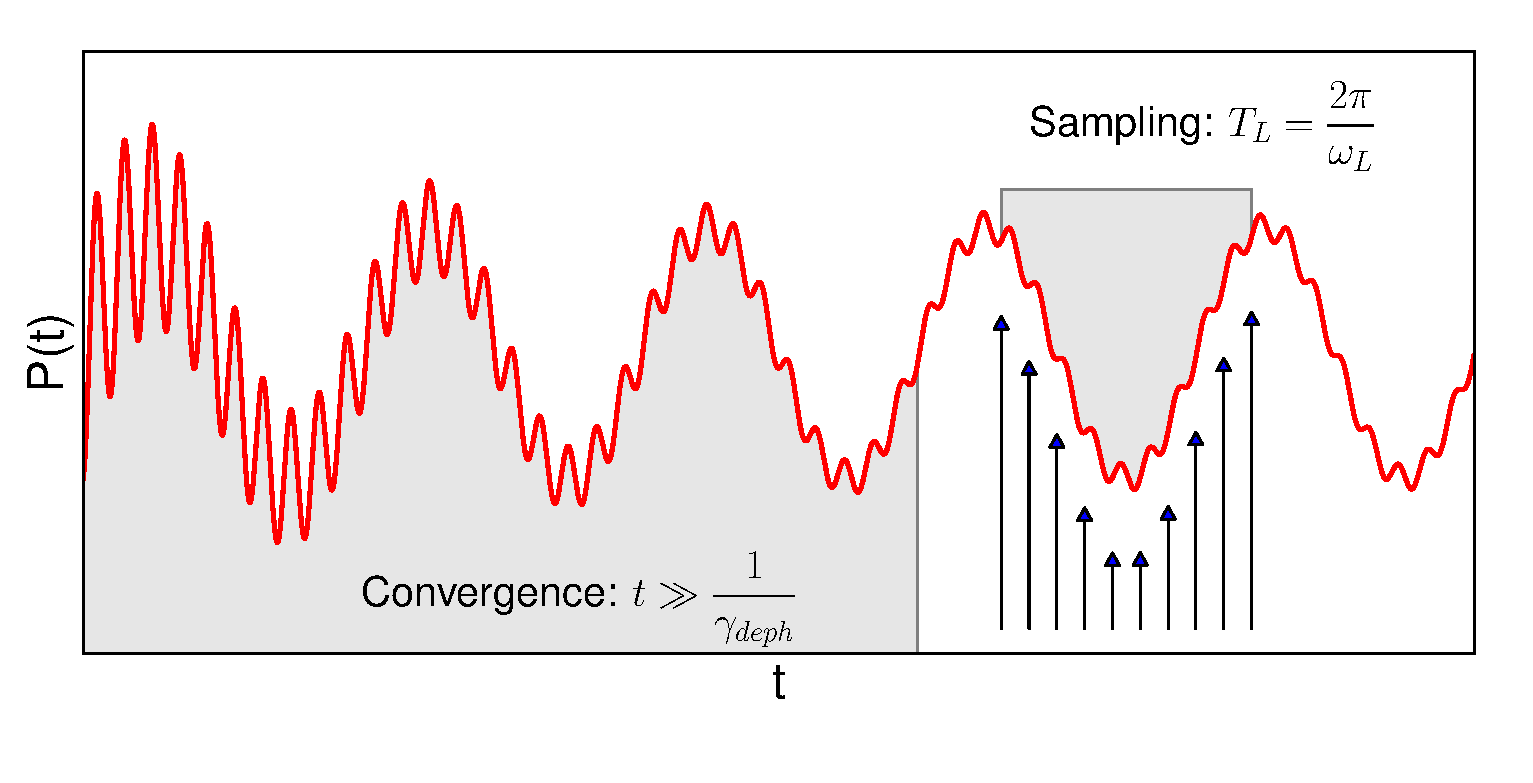
\includegraphics[width=0.5\textwidth]{Figures/Pt_analysis}
\caption{\footnotesize{Pictorial representation of the signal analysis in the post-processing step. The signal  $P(t)$ (red line) can be divided into two regions: an initial convergence region (up to $t\gg 1/\gamma_{deph}$) in which the eigenfrequencies of the systems are ``filtered out'' by dephasing. In this second region the signal $P(t)$ is sampled within a period $T_L=2\pi/\omega_L$ to extract the $\pp_n$ coefficients. %Note that $P(t)$ is not a realistic one: for illustration purposes we enhanced the second-harmonic signal that otherwise would not be visible on this scale. 
	\label{fg:ptanalysis} }} 
%\end{figure} 
\end{wrapfigure}
When the wave-function cannot be approximated anymore with a single Slater determinant (as in strong-correlated systems) the evaluation of the polarisation operator [Eq.~\ref{limit} ] becomes quite cumbersome.\cite{stella} Also we are not aware of any successful attempt to combine Berry's phase polarisation with Green's function theory or density matrix kinetic equations beyond the screened Hartree-Fock approximation (i.e. including scattering terms), even if some appealing approaches have been proposed in the literature\cite{restagw,PhysRevB.84.205137,doi:10.7566/JPSJ.83.033708,nourafkan2013electric}.\\
Notice that all correlation terms we included in the Hamiltonian, Eq.~\ref{mbhamiltonian}, are Hermitian and static, therefore they do not provide any dephasing effect in the dynamics. In order to describe dephasing due to electronic correlation, scattering with phonons and broadening from other sources, we included a phenomenological non-Hermitian operator as described in Ref.~\onlinecite{nloptics2013}. The latter approach to include dephasing effects are formally correct for non-interacting electrons. A proper formulation of dephasing beyond the IPA is instead far from trivial within single particle approaches (either density-matrix or wave-function based).\cite{sangalli2021excitons}
%
% SUB EXACT WITH FORMALLY CORRECT. HOW CAN BE A PHENOMENOLOGICAL TERM 'EXACT'?
%

%time-dependent screened Hartree-Fock (TDSHF),\cite{strinati} where the single particle energies have been shifted to reproduce the $G_0W_0$ quasiparticle band structure. ADD SOME EQUATIONS
%% Correlation among electrons can be included at different level of accuracy. As starting point we consider a system of independent particle where the energy levels have been renormalized by the electron-electron interaction:
%% \bea
%% i\hbar  \frac{d}{dt}| v_{\kk,m} \rangle &=& (\HH^0_{\kk} + \Delta \HH_{\kk}) | v_{\kk,m} \rangle \nonumber \\ &+& ie \efield \cdot| \partial v_{\kk,m} \rangle. \label{tdbse_ip}
%% \eea
%% The $\Delta \HH_{\kk}$ operator is the so-called the scissor operator that can be calculated \ai or introduced by hand, $\HH^\kk_0$ is the Kohn-Sham Hamiltonian.\\
%% Beyond the independent quasi-particles it is possible to include correlation effects in the response. First of all we consider the fluctuations of the density. The external field induces a variation of the density that in turn generates an additional potential through the Hartree term:
%% \bea
%% i\hbar  \frac{d}{dt}| v_{\kk,m} \rangle &=& (\HH^0_{\kk} + \Delta \HH_{\kk}) | v_{\kk,m} \rangle \nonumber \\ &+& V_h(\Delta \rho)+ ie \efield \cdot| \partial v_{\kk,m} \rangle \label{tdbse_hartree}\\
%%  \rho(\mathbf r) &=& \frac{1}{N_\kk} \sum_{\kk,m} \langle r | v_{\kk,m} \rangle \langle v_{\kk,m} | r \rangle \nonumber
%% \eea
%% where $\Delta \rho=\rho-\rho_0$ is the variation of the density induced by the external perturbation. Notice that the linear response limit of the time-dependent Hartree reduce to the called local field effects.\cite{PhysRev.126.413} The first term beyond the Hartree one is generated by the exchange between electrons. We include exchange and correlation effects within the time-dependent screened Hartree-Fock (TDSHF)\cite{strinati} approximation:
%% \bea
%% i\hbar  \frac{d}{dt}| v_{\kk,m} \rangle &=& (\HH^0_{\kk} + \Delta \HH_{\kk}) | v_{\kk,m} \rangle \label{tdbse_shf}  \\ &+& V_h(\Delta \rho) \nonumber + \Sigma_{sex} (\hat \rho -\hat \rho_0 ) + ie\efield \cdot | \partial v_{\kk,m} \rangle \nonumber \\
%% \hat \rho &= & \sum_{\kk,m}  | v_{\kk,m} \rangle \langle v_{\kk,m} | \nonumber 
%% \eea
%% In the screened exchange we keep the screening fix to its initial value, while we update the density matrix $\hat \rho$ at each step of the dynamics, for more details see ref.~\cite{attaccalite}. In this article we will present results only with Eq.~\eqref{tdbse_ip} and \eqref{tdbse_hartree}. In fact even if TDSHF is not difficult to implement, it is very computer demanding\cite{attaccalite} and we are developing advanced techniques to speed up Eq.~\eqref{tdbse_shf} that will be discussed in a sequent paper.\\
%% 
% 
\subsubsection{Density-polarization functional theory formulation}\label{ss:dfpt}
%Density functional theory (DFT)\cite{PhysRev.140.A1133,PhysRev.136.B864} is a standard approach for calculating ground-state properties of extended and finite systems\cite{doi:10.1021/jp960669l,RevModPhys.87.897}. Time-dependent density functional theory (TDDFT) is an extension of the ground-state formalism that allows to investigate the properties and dynamics of many-body systems in the presence of time-dependent potential. TDDFT is based on the Runge-Gross (RG) theorem\cite{PhysRevLett.52.997}  that establishes a one-to-one correspondence between time-dependent densities and time-dependent one-body potentials. For example when we consider an isolated molecule and an electric filed as  perturbation by means of TDDFT we have access its optical response. As for the DFT case, the RG theorem just guarantees the existence of the mapping, but do not provide a way to construct it. Different approximations for the time-dependent (or frequency dependent) exchange-correlation functional have been proposed in the literature. Exchange correlation functional have been obtained from the ones of the DFT, including long range corrections or derived from more accurate methods\cite{Onida,faber2014excited}. The response equations of TDDFT have been encoded in standard quantum chemical packages\cite{valiev2010nwchem}, and real-time TDDFT is currently used to simulate the short time dynamics of excited electrons\cite{PSSB:PSSB200642067}.\\
As discussed previously, the time-dependent density functional theory (TDDFT)  is an approach to calculate optical properties beyond the IPA.
% An alternative way to BSEinclude correlation effects in the 
TDDFT is an extension of the ground-state formalism that allows to investigate the properties and dynamics of many-body systems in the presence of time-dependent potential.\cite{PhysRevLett.52.997} 
TDDFT has been applied successfully in molecular systems. In contrast with other approaches, as for instance Green's function theory\cite{strinati} that provides a similar accuracy in extended\cite{Aulbur19991} and finite systems\cite{li2019comparing}, results obtained within standard TDDFT for dielectrics has an accuracy similar to the Random Phase Approximation.
On the other hand, TDDFT has a much lower cost than the Green's function formalism and it is therefore appealing to develop TDDFT approaches that, maintaing the computational costs of standard approximations, can provide accurate optical spectra of dielectrics.   
\begin{wrapfigure}{l}{0.4\textwidth}
%\begin{figure}[ht]
\centering
\epsfig{figure=Figures/SiC_absX2_QPRPA_vs_Luppi_half.pdf,width=0.4\textwidth,clip}
\caption{\footnotesize{Magnitude of $\chi^{(2)}(-2\omega,\omega,\omega)$ for bulk SiC calculated within the IPA (black triangles) and QPA (red circles). Each point corresponds to a real-time simulation at the given laser frequency. Comparison is made with results obtained \ai by direct evaluation of the $\chi^{(2)}$ in Ref.~\cite{PhysRevB.82.235201} in IPA (grey solid line) and QPA (brown dashed line).  \label{fg:SiCQPRPA} }}
%\end{figure}
\end{wrapfigure}

While much of the attention in the literature is dedicated to the development of approximations for the exchange-correlation potential---that effectively describes many-body effects within DFT, the issue of TDDFT in solids is of fundamental nature. The central proof of TDDFT, demonstrating the mapping between the time-dependent density and the time-dependent potential, relies on the mapping between currents and densities through the continuity equation. This mapping requires a surface integral involving the density and the potential to vanish. For finite systems, this condition is satisfied rigorously. For a periodic system, the condition can be satisfied as long as the density and potential are periodic. When a macroscopic uniform electric field is applied and the potential is no longer periodic, there is no mapping between density and current-density and TDDFT does not apply.\cite{Gonze1995} This is exactly the case when we try to calculate optical properties by using TDDFT. 

A nice illustration of this fundamental problem is given in the paper of Maitra et. al.\cite{maitra2003current} through the example of a free electron gas on a ring subjected to a constant uniform electric field. For this simple system, it is possible to write down the exact solution: one finds that the electric field modifies only the phase of the single particle orbitals, leaving the density unchanged. Then different electric fields  give rise to exactly the same density and therefore there is not an unique mapping between the density and the (macroscopic) external field.  The problem can be overcome considering instead the mapping of the macroscopic external field with current density. In fact, an extension of TDDFT, Time-Dependent Current Density Functional Theory (TD-CDFT)---that maps directly the external potential and the current-density---was proposed at by Ghosh and Dhara in the late eighties~\cite{PhysRevA.38.1149}. 

An alternative to the current density based TD-CDFT is the density and polarization based time-dependent density and polarization functional theory (TDDPFT). In the latter approach, one uses the relation between polarisation and current to construct a theory that relies on density and polarization instead of current density. The use the polarisation as an additional to the density is a valid approximation when the transverse microscopic contribution of the current is negligible. In the case of the optical response in the limit of long-wave length limit, this is a valid approximation. Within the TDDFTP the Hamiltonian reads:
\be \label{eq:dpftks}
H^{s}_\kk
= -\frac{1}{2}\left(\nabla + i\kk\right )^2 + \bar v^{s}(\rr) -\Omega\Efield^{s}\cdot \nabla_\kk %CHECK
\ee
which is a functional of both the density and the polarisation and $\Efield^{s}$ is the Kohn-Sham (KS) macroscopic field, that contains the corresponding macroscopic components of the exchange correlation functional. The KS macroscopic electric field can be parameterised in different way, starting from long-range corrected functionals, imposing the exact constraint in the linear response limit. We tested and implemented different possible approximations for the KS macroscopic electric field, see Refs.~\onlinecite{gruningtddf1,gruningtddf2}.


\subsubsection{Non-linear response functions from real-time simulations}\label{sc:compdet}

A real-time simulation outputs the real-item polarisation. Similarly to an experiment, we can change the intensity and temporal behaviour of the external field and the signal post-processing to obtain the response function of interest.      
%In previous sections we have shown how to obtain EOMs in length gauge in extended systems and how to include correlation effects, here we discuss how to extract different non-linear response functions from real-time simulations.\\
For example in the second/third harmonic generation case, we perturb the system with a monochromatic electric field $\efield(t) = \efield_0 \sin(\omega_L t)$, where $\omega_L$ is the frequency of the external perturbation. Once due to decoherence, the amplitude of the eigenemodes of the system becomes negligible, the polarisation $\PP(t)$ is a periodic function of period $T_L =\frac{2\pi}{\omega_L}$ and can be expanded in a Fourier series as:
\be
\PP(t) = \sum_{n=-\infty}^{+\infty} \pp_n e^{-i n \omega_L t}, 
\label{eq:chifromp}
\ee
 where the complex coefficients $\pp_n$ are proportional to the $n^{th}$-harmonic-generation response at $\omega_L$. These coefficients can be obtained by solving the set of linear equations resulting when Eq.~\ref{eq:chifromp} is truncated at some order $N$ and evaluated at $2N+1$ times $t$ sampled as shown in Fig.~\ref{fg:ptanalysis}.  %fitting the polarization with the above functional form, as show in Fig.~\ref{fg:ptanalysis}. % IT IS NOT A FIT! 
To obtain the frequency-dependent  $n^{th}$-harmonic-generation response, one runs a set of simulations sweeping $\omega_L$ over the range of frequencies of interest. 
 
\begin{wrapfigure}[19]{r}{0.5\textwidth}
    \centering
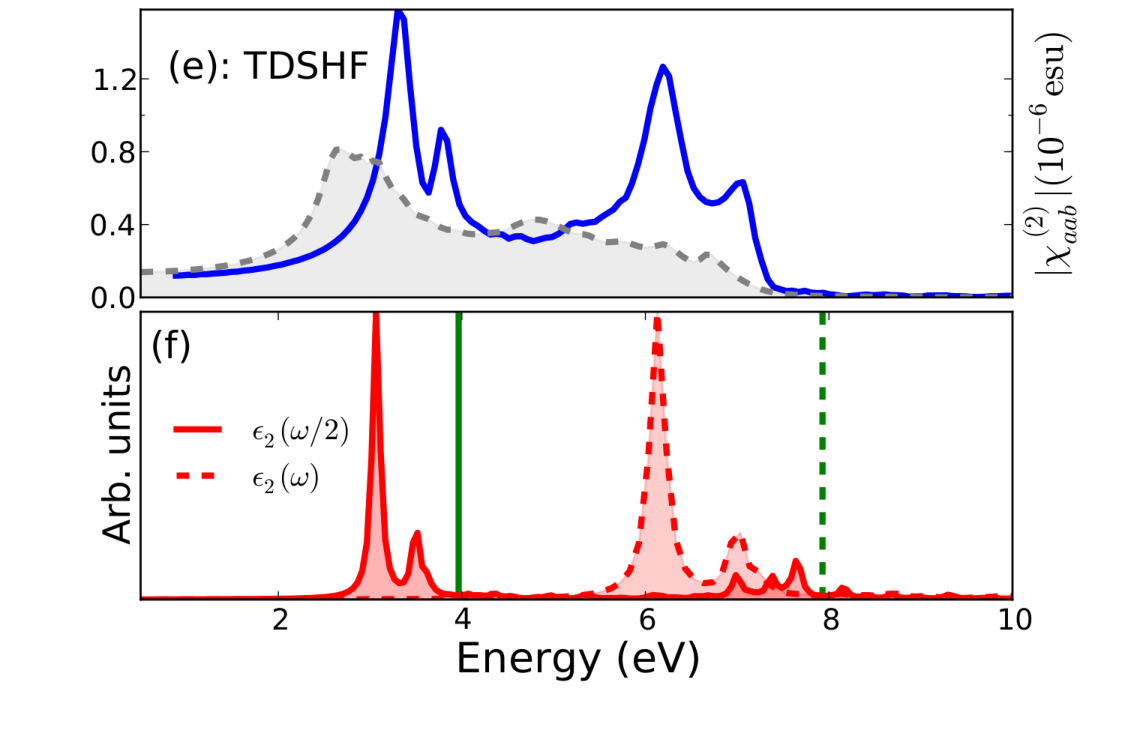
\includegraphics[width=0.5\textwidth]{Figures/eps_and_X2_short}
	\caption{\footnotesize{SHG spectra for the h-BN monolayer at different levels of theory [Eq.~\eqref{mbhamiltonian}]: (a) IPA (dashed grey line) and TD-BSE (continuous blue line). The imaginary part of the dielectric constant at both $\omega/2$ (red continuous line) and $\omega$ (red dashed line) is reported in (b) at the  TD-BSE level. The vertical lines represent the $GW$ fundamental gap (green dashed line) and half of the $GW$ fundamental gap (green continuous line). \label{X2bn} }}
%\end{figure}
\end{wrapfigure}

A different scheme is used to study the two-photon absorption.  Two-photon absorption is given by the third-order response function at the same frequencies of the incoming laser. In this case, for a given laser frequency, we perform simulations at different laser intensities and we resort to a Richardson extrapolation to extract the contribution we are interested in.\cite{attaccalite2018two}

\subsection{Results}\label{sc:results}
The computational scheme presented in previous sections has been used to calculate nonlinear properties in a range of systems. 

First, the computational approach has been validated by direct comparison with existing calculations in frequency domain for bulk semiconductors. For example in Fig.~\ref{fg:SiCQPRPA} we compare SHG in SiC calculated from real-time simulations against the results of Refs.~\cite{PhysRevB.82.235201,PSSB.427.1984}. An almost perfect agreement between the two approaches was found. Similar comparison has been performed also for third harmonic generation against simple models and against experimental results, see Ref.~\onlinecite{nloptics2013}.\\
The approach has been used particularly for 2D and layered materials\cite{attaccalite2015strong,wei2019second,beach2020strain,mishra2020exciton,attaccalite2019second} for which non-linear optical properties are dominated by strongly bound excitons, that as discussed previously are not captured by other approaches. As an example, we show the non-linear response of h-BN. In Fig.~6
%\ref{X2bn}
we report the calculated absolute value of $\chi^{(2)}_{aab} (\omega)$ at different levels of approximation. 
%$\chi^{(2)}_{aab} (\omega)$, where $a$ and $b$ are the in-plane Cartesian directions, is the only independent in-plane component of $\chi^{(2)} (\omega)$: all other components can be obtained from the $\chi^{(2)}_{aab} (\omega)$ with simple symmetry considerations, for instance $\chi^{(2)}_{bbb} (\omega)=-\chi^{(2)}_{aab} (\omega)$. 
At IPA level, the SHG presents a peak at $2.3~eV$ and a broad structure between $4 - 7 eV$. When we turn on correlation effects using the full Hamiltonian, Eq.~\eqref{mbhamiltonian}, the results change completely.
Excitonic effect enhance the non-linear response and compensate the quasi-particle corrections. By comparing with the imaginary part of the dielectric constant $\epsilon_2$ both at $\omega/2$ and  $\omega$ [Fig.~6] calculated at the same level of theory, the two couples of peaks can be identified respectively as the two- and one-photon resonances with the excitons at $6$ and $7~eV$. 
Excitonic effects has been studied also for the two-photon absorption in single layered and bulk h-BN and for the third-harmonic generation of one-dimensional systems, see Ref.~\onlinecite{attaccalite1d,attaccalite2018two}. In the latter case, adding quasiparticle corrections and excitonic effects leads again to a very different spectra when compared to the independent particle case. In particular, there is a strong redistribution of the intensity over a broader range of frequencies, with the net result of a reduced intensity of the main peak with respect to the IPA.\\ 
SHG spectrum of semiconductors have been treated as well within the TD-DPFT framework\cite{PhysRevB.82.235201} by using the so-called long-range-corrected (LRC) approximation,\cite{LRC} a semi-empirical simple model for the screened electron-hole attraction, that includes only the long-range part of the interaction. %In Fig.~6 we see the $\epsilon_2$ calculated within the LRC approximation: 
As earlier recognised, this approximation fails for strong excitons. In fact by tuning the empirical parameter for the screening we could get the position of the first exciton, though its intensity is strongly overestimated (see caption of Fig.~6), but in no way we could get the second excitonic peak. Those pitfalls reflected also in the SHG spectrum, as shown in Refs.~\cite{gruningtddf1,gruningtddf2}. 

\section{Conclusions}\label{conclusion}                                        
In this highlight we presented an \ai real-time approach to calculate nonlinear optical properties of extended systems in the length gauge. The key strengths of the proposed approach are first, the correct treatment of the coupling between electrons and the external field and second the possibility to include easily static correlation effects beyond the IPA.
This approach is implemented in the Yambo code\cite{yambo} and different tutorials are available on how to calculate the non-linear response.\cite{yambo_wiki} The code is open-source and freely available.% ADD REF TO GITHUB REPO?
The code avails of the sophisticated parallelization of the yambo code\cite{yambo} and allows to parallelize the simulations on frequencies and $\kk$-points. 
%
% THREADS???? I DON'T THINK THIS WAS CLEAR - NOT TO ME - EITHER NEEDS TO BE EXPLAINED BETTER OR LEAVE IT OUT
%

Although very accurate for the non-linear response, our approach is missing dynamic correlation effects, to accurately describe scattering and decoherence, processes and correlation effects beyond electron-hole interaction, as for example those needed to describe bi-excitons or trions.\cite{schafer} Furthermore, calculation of non-linear response in complex system can be challanging due to the computational and memory requirements. 
There are several on-going efforts to extend the approach and overcome some of its limitations, for example, 1) the extension to pump and probe spectroscopies; 2) the inclusion of temperature effects by considering an electron-phonon self-energy; 3) the application to non-perturbative phenomena as high-harmonic generation.


%Regarding the treatment of the electron-field coupling, following the work of Souza et al.\cite{souza_prb}, we started from the Berry's phase formulation for the dynamical polarisation---a definition consistent with the periodic boundart conditions (PBC)---to derive a covariant numerical expression for the dipole operator in the EOMs.

%ote that we worked in the length-gauge even if the velocity gauge may appear a more natural choice. In fact, as opposed to the position operator the velocity operator is consistent with the PBC. However, in the velocity gauge even if the position operator disappears from the Hamiltonian, it reappears in the phase factor for the wave-function~\cite{PhysRevA.36.2763}, so that the problem of re-defining the position operator remains. 
%Furthermore, the velocity gauge is plagued by unphysical numerical divergences for the response at low frequencies~\cite{PhysRevB.52.14636}. 
%	As an example, in the present chapter we have included quasi-particle corrections to the band-gap by adding to the Hamiltonian a scissor operator and crystal local-field effects by adding the time-evolution of the Hartree potential. In principle, one can add as well excitonic effects by adding the time-evolution of the screened exchange self-energy (see chapter~\ref{chaptercorr}); or perform a real-time TD-DFT calculations by adding the time-evolution of the exchange-correlation potential. Being the focus of this chapter the validation of the proposed approach for calculating nonlinear properties, the inclusion of these correlation effects is discussed in the rest of this work.
%We have proved the validity of our approach by comparing our results, obtained from real-time simulations, with results in the literature obtained from direct evaluation of the second order susceptibility in frequency-domain.  

